%==============================================================================
\chapter{Hawking Radiation}
\label{chap:hawrad}
%==============================================================================

%------------------------------------------------------------------------------
\section{$(3+1)$-dimensional Einstein gravitation}
\label{sec:hawrad-einstein}
%------------------------------------------------------------------------------

Based on the advances in the geometry of space-time and `mechanics' of black 
holes, as well as in quantum field theory in curved space-time, 
\citeauthor{HAWKING1974} quantitatively revealed a semi-classical property of 
the black holes in \cite{HAWKING1974}. In his model, the Einsteinian 
gravitational 
background is fixed to be that of a spherically collapsing body\footnote{A 
detailed account for space-times of collapsing body can be found in 
\cite{Joshi2007}.}, the conformal diagram of which is shown in 
\cref{fig:sph-col-bod}. A neutral (real), massless scalar field $\rfun{\phi}{x}$ 
is minimally coupled to the gravitational background, so the action of the model 
reads
\begin{equation}
S \coloneqq \int_{\mscrM} {\dd^4 x} \,\sqrt{-g}\,
\cbr{g^{\mu\nu}\rbr{\partial_\mu \phi}\rbr{\partial_\nu \phi}}.
\end{equation}
One quantises the scalar field canonically on the Cauchy surface $\mscrI^-$ by 
introducing ladder operators $a^\mp$'s, and on $\mscrI^+ \cup \mscrH^+$ by 
$b^\mp$'s (for $\mscrI^+$) and $c^\mp$'s (for $\mscrH^+$). An \emph{early-time 
vacuum} is defined by
\begin{equation}
	\rfun{a^-}{p}\Ket{h} \coloneqq 0,
\end{equation}
where $\rfun{a^-}{p}$ annihilates a particle with momentum $p$, so that
\begin{equation}
\abr{\rfun{{n}_a}{p}}_h \coloneqq \Braket{h | \rfun{{n}_a}{p} | h} 
\equiv 0,\qquad \forall p,
\end{equation}
where $\rfun{n_a}{p} = \rfun{a^+}{p}\rfun{a^-}{p}$ is the number operator of 
mode with momentum $p$. This means that an asymptotic observer at early time, 
whose definition of particles agrees with $a^\mp$, detects no particle.

\begin{figure}
\begin{center}
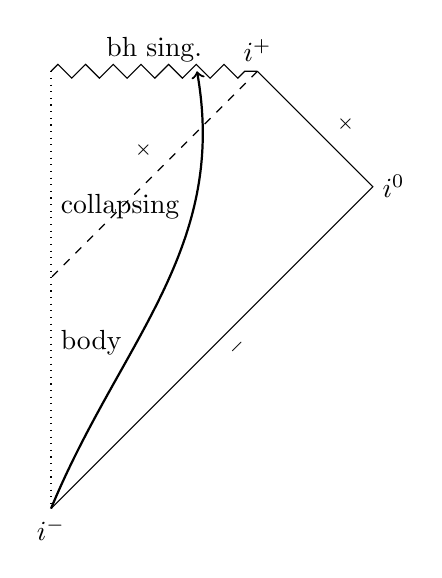
\begin{tikzpicture}%[scale=2]
\pgfmathsetmacro\myunit{3} 
\pgfmathsetmacro\sc{1.41421 35623 73095 04880 16887 24209 69807 85696 71875}
\pgfmathsetmacro\grs{0.6180339887498949}
\pgfmathsetmacro\grb{1.6180339887498949}
	\draw [decorate, decoration=zigzag] (0,0)
		-- ++ (+  0: \sc * \grs * \myunit)
			node [above] {$i^+$}
			node [pos = .5, above] {bh sing.}
			coordinate (i+);
	\draw [dotted] (0,0)
			\pgfextra{\pgfmathparse{(\grs/\sc+\sc)*\myunit}}
		-- ++ (- 90: \pgfmathresult)
			node [below] {$i^-$}
			node [pos = .31, right] {collapsing}
			node [pos = .62, right] {body}
			coordinate (i-);
	\draw (i+)
		\pgfextra{\pgfmathparse{(1 - \grs/2)*\myunit}}
		-- ++ (- 45: \pgfmathresult)
			node [right] {$i^0$}
			node [pos = .5, above right, sloped] {$\mscrI^+$}
			coordinate (i0)
		-- (i-)
			node [pos = .5, below right, sloped] {$\mscrI^-$};
	\draw [dashed] (i+)
		-- ++ (-135: 2 * \grs * \myunit)
			node [pos = .4, above left, sloped] {$\mscrh^+$};
	\draw [thick, out = 67.5, in = -80, thick, ->] (i-)
			to (\grs * \myunit, 0);
\end{tikzpicture}

\end{center}
\caption[Spherically collapsing body in Einstein gravitation]{A schematic 
conformal diagram of a spherically collapsing body in Einstein gravitation, in 
which massive matter (presumably a star) spherically collapses by gravitational 
interaction. The boundary of the collapsing body is denoted by the thick
line with arrow. The quantum field is solved on $\mscrI^-$ and $\mscrI^+ \cup 
\mscrh^+$. \label{fig:sph-col-bod}}
\end{figure}

For asymptotic observers, \citeauthor{Hawking1975} was able to evaluate the 
\emph{late-time} properties, or those with respect to the $b$'s, of 
$\Ket{h}$. He derived in \cite{Hawking1975} that\footnote{Possible divergent 
$\rfun{\delta}{0}$ factors in the particle-number expectations have been 
systematically ignored.}
\begin{equation}
\abr{\rfun{{n}_b}{\omega}}_h \approx
\Gamma_\omega\rbr{\ee^{2\pp\omega/\kappa}-1}^{-1},
\label{eq:hawking-distri}
\end{equation}
where $0 < \Gamma_\omega < 1$ is the \emph{grey-body factor}, and $\omega$ 
being the angular frequency of the mode regarded. Comparing 
\cref{eq:hawking-distri} with that of a Bose--Einstein distribution, or a 
\emph{black-body} radiation field,
\begin{equation}
\abr{\rfun{{n}}{\omega}}_\text{BE} = \rbr{\ee^{\omega/T} - 1}^{-1},
\end{equation}
it is appealing to conclude that \cref{eq:hawking-distri} describes a 
\emph{grey-body} radiation field, with the temperature
\begin{equation}
T_\text{H} \coloneqq \kappa/2\pp \equiv \phs/\lc \bk \cdot \kappa/2\pp,
\label{eq:hawking-temperature}
\end{equation}
also named after \citeauthor{Hawking1975}, and an absorption coefficient 
$\Gamma_\omega$.

\citeauthor{Hawking1975} himself argued that his calculation also holds for 
a matter field with spin, as well as for the collapse result being a rotating 
black hole. Further quantities could also be obtained in the background of 
an eternal black hole, whose connection to an astrophysical collapsing body 
has been constructed, showing the evaluation is physically robust 
\cite{Candelas1980}. The algebraic approach to quantum fields showed that it is 
also mathematically reliable \cite{Hollands2015}.

Though widely acknowledged, Hawking temperature is in fact technically 
ill-defined, if we take the calculation \emph{seriously enough}. Recall that a 
temperature $T$ of a quantum system can only be defined if the system is in a 
thermal equilibrium, which can be described by a density operator
\begin{equation}
	\rho = Z^{-1} \ee^{-H/T}
\end{equation}
of a \emph{mixed state}, where $H$ is the Hamiltonian of the system, and $Z = 
\tr\ee^{-H/T}$ is the partition function. For a bosonic system, the density 
operator reads
\begin{equation}
{\rho}_\text{BE} \sim Z^{-1} \sum_E \ee^{-E/T} \Ket{E}\Bra{E},
\label{eq:bos-ein-dis}
\end{equation}
where $\rbr{E, \Ket{E}}$ are the energy eigenvalue and the corresponding 
eigenstate of the system, respectively. As $\Ket{h}$ is a \emph{pure state}, 
whose density operator reads
\begin{equation}
\rho_h \coloneqq \Ket{h}\Bra{h},
\label{eq:haw-den-optr}
\end{equation}
it is drastically different from \cref{eq:bos-ein-dis}. One naturally asks, how 
different are the pure and mixed states, and what does it imply?

%------------------------------------------------------------------------------
\section{In $(1+1)$-dimensional dilaton gravity}
\label{sec:hawrad-1+1dila}
%------------------------------------------------------------------------------

In the Einsteinian background of a collapsing body, in which 
\citeauthor{HAWKING1974} did his calculation, no analytic solution of a quantum 
field theory has so far been found due to technical difficulties. To study the 
problem in more detail, alternative solvable gravity models can be used, which 
may help understanding the quantum aspects of Einstein gravitation. Here a 
gravity model in $\rbr{1+1}$ space-time dimensions with a dilaton field is 
adapted, which is further explained in \cref{sec:1+1ddlt}. The solution with a 
collapsing null-matter-shell in such a model, also known as the 
CGHS\footnote{Introduced by \citeauthor{Callan1992} in \cite{Callan1992}.} black 
hole, has been found at the classical level and can also be formally quantised 
canonically \cite{Callan1992,Demers1996}. The conformal diagram of the classical 
solution is shown in \cref{fig:dil-col-bod}.

\begin{figure}
\begin{center}
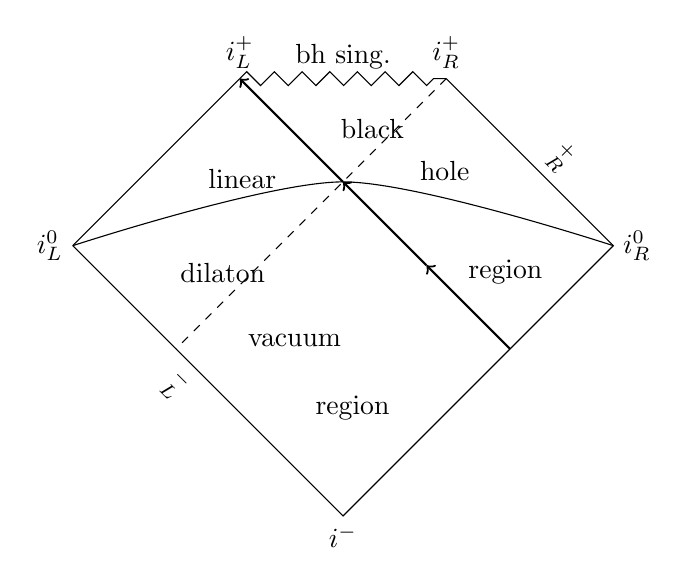
\begin{tikzpicture}%[scale=2]
\pgfmathsetmacro\myunit{3}
\pgfmathsetmacro\grs{0.6180339887498949}
\pgfmathsetmacro\grb{1.6180339887498949}
	\draw (0,0)
			node [left] {$i^0_\text{L}$}
		-- ++ (- 45: \grb * \myunit)
			node [pos = .50, below left, sloped] {$\mscrI^-_\text{L}$}
			node [pos = .10, right = .3*\myunit cm] {dilaton}
			node [pos = .35, right = .3*\myunit cm] {vacuum}
			node [pos = .60, right = .3*\myunit cm] {region}
			node [below] {$i^-$}
		-- ++ (+ 45: \myunit)
			%node [above = .25*\myunit cm] {region}
			coordinate (one)
		-- ++ (+ 45: \grs * \myunit)
			node [pos = .75, left = .15*\myunit cm] {region}
			node [right] {$i^0_\text{R}$}
			coordinate (r-inf)
		-- ++ (+135: \myunit)
			node [pos = .70, left = .35*\myunit cm] {black}
			node [pos = .45, left = .25*\myunit cm] {hole}
 			node [pos = .50, above right, sloped] {$\mscrI^+_\text{R}$}
			node [above] {$i^+_\text{R}$}
			coordinate (r-i+)
			;

	\draw (0,0)
		-- ++ (+ 45: \myunit)
			node [pos = .4, right = .25*\myunit cm] {linear}
			node [above] {$i^+_\text{L}$}
			coordinate (l-i+);
			%node [below = .55*\myunit cm] {linear}
			%node [below = .75*\myunit cm] {dilaton}
			%node [below = .95*\myunit cm] {vacuum};

	\draw [dashed] (r-i+)
		-- ++ (-135: \grb * \myunit)
			coordinate (mlambda);
		
	\draw [thick, ->] (one)
		-- ++ (+135: 0.5 * \myunit)
			coordinate (bb);
	\draw [thick, ->] (bb)
		-- ++ (+135: 0.5 * \myunit)
			coordinate (cross);
	\draw [thick, ->] (cross) -- (l-i+);

	\draw [decorate, decoration=zigzag] (l-i+)
		-- (r-i+)
		node [pos = .5, above] {bh sing.};

	\draw plot [smooth, dash dot] coordinates {(0,0) (cross) (r-inf)};
\end{tikzpicture}
\end{center}
\caption[Collapsing null matter in dilaton gravity]{The conformal 
diagram of collapsing null shell in $\rbr{1+1}$ dimensional dilaton gravity. 
The black-hole horizon is marked by the dashed line, whereas the ingoing null 
shell is expressed by the thick line with arrow. The \emph{linear dilaton 
vacuum region} and the \emph{black hole region} mark the space-time blocks 
before and after the ingoing shell, respectively. The quantum field, on the 
other hand, is solved on the hyper-surface connecting $i^0_\text{L/R}$ and the 
intersection of the null shell and the horizon.
\label{fig:dil-col-bod}}
\end{figure}

At the next-to-leading order in the semi-classical approximation scheme, the 
matter field can be separated from the gravity and the dilaton, and a quantum 
theory of fields in curved space-time can be \emph{derived} in terms of a 
functional Schrödinger equation
\begin{equation}
	\ii \frpa{\sfun{\chi}{f}}{t} = \int \dd x\,\frac{1}{2}
	\cbr{-\frdva{^2}{f^2} + \rbr{\frpa{f}{x}}^2} \sfun{\chi}{f},
\label{eq:functional-Sch-chi}
\end{equation}
where $\rfun{f}{x}$ is the classical matter field promoted to an operator, and 
$\sfun{\chi}{f}$ the corresponding matter wave-functional. Before the collapse 
of the ingoing null-matter-shell where the region is called \emph{linear dilaton 
vacuum}, a `vacuum' state can be found, whose wave functional reads
\begin{equation}
	\sfun{\chi_0}{f} \propto
	\cfun{\exp}{-\frac{1}{2}\int_{0}^{+\infty}\dd k\, k \, \rfun{f}{k}^2},
\label{eq:vacuum-wave-functional-f}
\end{equation}
where $\rfun{f}{k}$ is the Fourier sine transform of $\rfun{f}{x}$. 
\Cref{eq:vacuum-wave-functional-f} is nothing else but a generalisation of the 
ground-state wave function of a simple harmonic oscillator, see 
\cref{chap:harosc}.

After the collapse where the region is called \emph{black hole}, the spacial 
slice is shifted, and so are the Fourier modes of the matter field. It can be 
shown that
\begin{equation}
	\rfun{f}{k} = \int_{-\infty}^{+\infty} \dd l\,
	\rfun{\alpha}{k;l} \rfun{g}{l}\qquad k > 0,
\end{equation}
where $\rfun{g}{l}$ is the Fourier transform of matter field after the ingoing 
shock wave. The Bogolyubov-type coefficient $\rfun{\alpha}{k;l}$ has been 
computed, substituting which into \cref{eq:vacuum-wave-functional-f} yields
\begin{equation}
\sfun{\chi_b}{g} \propto 
\cfun{\exp}{-\int_{-\infty}^{+\infty}\dd p\, p \,\rfun{\coth}{\frac{\pp 
p}{2\lambda}} \vbr{\rfun{g}{p}}^2}
\label{eq:squeezed-wave-functional}
\end{equation}
in the black hole region, which is a squeezed-state wave functional 
\cite{Kiefer2001} and obviously different from a ground-state wave 
functional. The particle-number expectation of 
\cref{eq:squeezed-wave-functional} reads
\begin{equation}
	\abr{\rfun{n}{k}}_{\chi_b} = \rbr{\ee^{2\pp\vbr{k}/\lambda} - 1}^{-1},
	\label{eq:particle-num-exp-dilaton}
\end{equation}
%\begin{equation}
%\rfun{g}{k} = \int_{-\infty}^{+\infty}\dd v\,
%\frac{\ee^{-\ii k v}}{\sqrt{2\pp}} \rfun{f}{v},
%\end{equation}
leading to a Hawking-like \emph{black-body} temperature
\begin{equation}
T_\text{HD} \coloneqq \lambda/2\pp.
\label{eq:hawking-dilaton-temperature}
\end{equation}
Here it is the cosmological constant $\lambda$ which takes the place of surface 
gravity $\kappa$ in \cref{eq:hawking-temperature}.

%------------------------------------------------------------------------------
\section{Discussion}
\label{sec:hawrad-discussion}
%------------------------------------------------------------------------------

Though used throughout this work, the density operators can be mathematically 
defined only when they are \emph{trace-class} for which a trace may be defined, 
and this is not proved for any of the cases concerned. Unfortunately, the 
density operators are often not trace-class, especially in quantum field 
theory. A rigorous approach to deal with such thermal states can be the 
Kubo--Martin--Schwinger state \cite{Kubo1957,Martin1959,Haag1967} defined in 
algebraic quantum theory, which is concisely introduced in 
\cite[ch.~3]{David2015}.

Alert readers may be concerned about the result 
\cref{eq:squeezed-wave-functional}, which is derived in dilaton gravity model, 
not from Einstein gravitation. The solution is believed to be physically 
relevant, not only because it gives a same Hawking-like temperature for the CGHS 
black hole. It has also been shown that the wave functional of a massless, 
neutral scalar field in the Unruh effect yields exactly the same particle-number 
fluctuation and Hawking temperature \cite{Freese1985,Kiefer2001}. People have 
argued and widely believed that the Unruh effect is closely connected to 
Hawking radiation in Einstein gravity, especially in the space-time region near 
the horizon (e.g.\ \cite{Susskind2004}). It is therefore reasonable to believe 
that the aforementioned results from the CGHS model give hints about reality.

%%% Local Variables: 
%%% mode: latex
%%% TeX-master: "../mythesis"
%%% End: 
